\section{Physical description of dispersed two phases flows}

In this section we present the problem at hand, along with all the relevant physical and dimensionless parameters.
Then we introduce the ranges of dimensionless parameters that correspond to our specific industrial problem. 
A representation of the situation is depicted \ref{fig:scheme} where we can observe droplets immersed in a continuous fluid phase.
The dispersed phase is Newtonian fluid defined by its viscosity $\mu_d$, and density $\rho_d$. 
The definition of $D^\alpha$ is such that it represents the diameter of a sphere with the same volume as the particle $\alpha$.
Note that we consider poly-disperse emulsion of deformable particles, therefore the quantity $D^\alpha$ is not necessarily the same for all particles.   
Nevertheless, we define the representative length scale of the dispersed phase as the averaged size of the droplets noted by $D$. 
The continuous phase is also a Newtonian fluid of viscosity and densities of respectively $\mu_c$ and $\rho_c$.  
We will consider one external body force, namely the gravity $\textbf{g}$. 
Finally, it should be noted that the surface tension coefficient at the interface between the dispersed and continuous phases is commonly referred to as $\sigma$.
\begin{figure}[h!]
    \centering
    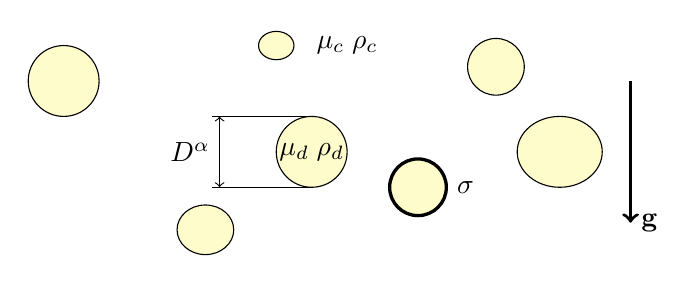
\begin{tikzpicture}[scale = 0.9]
        \draw[fill=yellow!20](3,3) node{$\mu_c\;\rho_c$};
        \foreach \x/\y/\ra/\r in {2/3/0.2/0.25,
        5.1/2.7/0.4/0.4,
        1/0.4/0.35/0.4,
        4/1/0.4/0.4,
        6/1.5/0.5/0.6,
        -1/2.5/0.5/0.5}{
            \draw[fill=yellow!20](\x,\y) ellipse(\r cm and \ra cm);
        }
        \draw[fill=yellow!20](2.5,1.5) circle(0.5)node{$\mu_d\;\rho_d$};
        \draw[thin,-](1.1,2)--++(1.4,0);
        \draw[thin,-](1.1,1)--++(1.4,0);
        \draw[very thick,black!80!black](4,1) ellipse (0.4cm and 0.4cm);
        \draw[very thick,black!80!black](4,1)++(0.4,0)node[right]{$\sigma$};
        \draw[thin,<->](1.2,1)--++(0,1)node[midway,left]{$D^\alpha$};
        \draw[very thick,->](7,2.5)--++(0,-2)node[right]{$\textbf{g}$};
    \end{tikzpicture}
    \caption{Scheme of droplets immersed into a continuous fluid phase.}
    \label{fig:scheme}
\end{figure}

There is a total of $9$ independent physical parameters to this problem (if we consider only the mean of the sizes $D$), they are all constituted by 3 fundamental units, a length, a mass and the time.
Therefore, according to Buckingham $\Pi$ theorem we can define a minimum of $9-3 = 6$ dimensionless numbers to describe the problem. 
Several options are available the selection is somewhat arbitrary, so we choose the following set of dimensionless numbers. 
The $4^{th}$ first parameters are linked to the physical properties of the emulsion, namely, 
\begin{align*}
    & Ga^2 =\frac{\rho_c(\rho_c - \rho_d) g D^3}{\mu^2_c}& 
    & Bo =\frac{(\rho_c - \rho_d) g D^2}{\sigma}&
    & \mu_r = \frac{\mu_c}{\mu_d}& 
    & \rho_r = \frac{\rho_c}{\rho_d}&
\end{align*}
And the two remaining parameters are related to the topology of the flow, 
\begin{align*}
    \phi = \frac{V_d}{V_c} & &
    N_b = \frac{6V_d}{\pi D^3}
\end{align*}
with $N_b$ is the number of droplets in the volume considered and $\phi$ the volume fraction of the dispersed phase.
The \textit{Galileo number} or \textit{Archimedes number}, is the ratio of the buoyancy forces over the viscosity forces, noted $Ga$.
Note that the \textit{Reynolds number}, defined by, $Re = \rho_c L U/\mu$, where $U$ is the characteristic velocity, is equivalent to the \textit{Galileo number} if we take $U = \sqrt{gL(\rho_c-\rho_d)/\rho_c}$ as the velocity scale.
$Bo$ is the \textit{Bond} or \textit{E\"otv\"os number}, it is the ratio between the buoyancy forces and surface tension forces. 
Note that $We = Bo/Ga^2$, with $We$ the \textit{Weber number} compares the viscous forces with capillarity forces.
Thus, $We$ describe the deformation of the droplets, as an example, above a critical value of the \textit{Weber number} a droplet will break due to hydrodynamical forces \citet{deike2022direct}. 
Lastly, $\mu_r$ and $\rho_r$ are respectively the density and viscosity ratios. 

To give a brief idea about the range of interest of those numbers in the industrial context, we take the example of an oil/water emulsion.
In the real processes the diameter of the droplets lies in the range $D = [10 \mu \text{m}, 1 \text{mm}]$.
The density and viscosity of water are approximately $\rho_c = 1000 \text{kg/m}^3$ and $\mu_c = 10^{-3}$.
The density and viscosity of oil are close to $\rho_d = 900 \text{kg/m}^3$ and $\mu_d = 10^{-2}$.
We consider the gravity acceleration on earth, thus it is $g= 9.81 \text{kg.m.s}^{-2}$.
The surface tension of the system oil/water is known to be approximately $\sigma = 50 \text{mJ/m}^2$ \citep{de2015gouttes}. 
We display the values of dimensionless parameters computed with those physical parameters in \ref{tab:parameters}.
\begin{table}[h!]
    \centering
    \caption{Dimensionless parameters for a water/oil emulsion.}
    \begin{tabular}{|c||c|c|c|c|c|}
        \hline&$Ga$&$Bo$&$\phi$&$\mu_r$&$\rho_r$\\ \hline
        \hline Oil/Water&$[0.03,30]$&$[10^{-6};10^{-2}]$&$[0,0.15]$&$0.1$&$1.111$\\ \hline
    \end{tabular}
    \label{tab:parameters}
\end{table}
We can note that the \textit{Galileo number} is rather low therefore can already state that it will be necessary to investigate the stokes flow limit. 
Likewise, The \textit{Bond number} is very low, meaning that the droplets are nearly spherical.
Consequently, in the following models and numerical simulations we must consider some cases with spherical particles. 
The viscosity and density ratio as well as the volume fraction do not permit any additional assumption on the flow. 
